%%
%% This is file `sample-sigconf-authordraft.tex',
%% generated with the docstrip utility.
%%
%% The original source files were:
%%
%% samples.dtx  (with options: `all,proceedings,bibtex,authordraft')
%% 
%% IMPORTANT NOTICE:
%% 
%% For the copyright see the source file.
%% 
%% Any modified versions of this file must be renamed
%% with new filenames distinct from sample-sigconf-authordraft.tex.
%% 
%% For distribution of the original source see the terms
%% for copying and modification in the file samples.dtx.
%% 
%% This generated file may be distributed as long as the
%% original source files, as listed above, are part of the
%% same distribution. (The sources need not necessarily be
%% in the same archive or directory.)
%%
%%
%% Commands for TeXCount
%TC:macro \cite [option:text,text]
%TC:macro \citep [option:text,text]
%TC:macro \citet [option:text,text]
%TC:envir table 0 1
%TC:envir table* 0 1
%TC:envir tabular [ignore] word
%TC:envir displaymath 0 word
%TC:envir math 0 word
%TC:envir comment 0 0
%%
%% The first command in your LaTeX source must be the \documentclass
%% command.
%%
%% For submission and review of your manuscript please change the
%% command to \documentclass[manuscript, screen, review]{acmart}.
%%
%% When submitting camera ready or to TAPS, please change the command
%% to \documentclass[sigconf]{acmart} or whichever template is required
%% for your publication.
%%
%%
\documentclass[sigconf,authordraft]{acmart}
%%
%% \BibTeX command to typeset BibTeX logo in the docs
\AtBeginDocument{%
  \providecommand\BibTeX{{%
    Bib\TeX}}}

%% Rights management information.  This information is sent to you
%% when you complete the rights form.  These commands have SAMPLE
%% values in them; it is your responsibility as an author to replace
%% the commands and values with those provided to you when you
%% complete the rights form.
\setcopyright{acmlicensed}
\copyrightyear{2018}
\acmYear{2018}
\acmDOI{XXXXXXX.XXXXXXX}
%% These commands are for a PROCEEDINGS abstract or paper.
\acmConference[Conference acronym 'XX]{Make sure to enter the correct
  conference title from your rights confirmation email}{June 03--05,
  2018}{Woodstock, NY}
%%
%%  Uncomment \acmBooktitle if the title of the proceedings is different
%%  from ``Proceedings of ...''!
%%
%%\acmBooktitle{Woodstock '18: ACM Symposium on Neural Gaze Detection,
%%  June 03--05, 2018, Woodstock, NY}
\acmISBN{978-1-4503-XXXX-X/2018/06}


%%
%% Submission ID.
%% Use this when submitting an article to a sponsored event. You'll
%% receive a unique submission ID from the organizers
%% of the event, and this ID should be used as the parameter to this command.
%%\acmSubmissionID{123-A56-BU3}

%%
%% For managing citations, it is recommended to use bibliography
%% files in BibTeX format.
%%
%% You can then either use BibTeX with the ACM-Reference-Format style,
%% or BibLaTeX with the acmnumeric or acmauthoryear sytles, that include
%% support for advanced citation of software artefact from the
%% biblatex-software package, also separately available on CTAN.
%%
%% Look at the sample-*-biblatex.tex files for templates showcasing
%% the biblatex styles.
%%

%%
%% The majority of ACM publications use numbered citations and
%% references.  The command \citestyle{authoryear} switches to the
%% "author year" style.
%%
%% If you are preparing content for an event
%% sponsored by ACM SIGGRAPH, you must use the "author year" style of
%% citations and references.
%% Uncommenting
%% the next command will enable that style.
%%\citestyle{acmauthoryear}

\usepackage{amsmath} 
\usepackage{subfigure}
\usepackage{subcaption}
\usepackage{booktabs} 
\usepackage{algorithm}
\usepackage{algpseudocode}
\usepackage[T1]{fontenc}
\usepackage{wrapfig}
% T1 fonts will be used to generate the final print and online PDFs,
% so please use T1 fonts in your manuscript whenever possible.
% Other font encondings may result in incorrect characters.
%
\usepackage{graphicx}


%%
%% end of the preamble, start of the body of the document source.
\begin{document}

%%
%% The "title" command has an optional parameter,
%% allowing the author to define a "short title" to be used in page headers.
\title{Avoiding Reranking in Blending of Large Language Models for Efficient Conversational Question Answering}

%%
%% The "author" command and its associated commands are used to define
%% the authors and their affiliations.
%% Of note is the shared affiliation of the first two authors, and the
%% "authornote" and "authornotemark" commands
%% used to denote shared contribution to the research.
\author{Ben Trovato}
\authornote{Both authors contributed equally to this research.}
\email{trovato@corporation.com}
\orcid{1234-5678-9012}
\author{G.K.M. Tobin}
\authornotemark[1]
\email{webmaster@marysville-ohio.com}
\affiliation{%
  \institution{Institute for Clarity in Documentation}
  \city{Dublin}
  \state{Ohio}
  \country{USA}
}

\author{Lars Th{\o}rv{\"a}ld}
\affiliation{%
  \institution{The Th{\o}rv{\"a}ld Group}
  \city{Hekla}
  \country{Iceland}}
\email{larst@affiliation.org}





%%
%% By default, the full list of authors will be used in the page
%% headers. Often, this list is too long, and will overlap
%% other information printed in the page headers. This command allows
%% the author to define a more concise list
%% of authors' names for this purpose.
\renewcommand{\shortauthors}{Trovato et al.}

%%
%% The abstract is a short summary of the work to be presented in the
%% article.
\begin{abstract}
Integrating responses from multiple large language models (LLMs) can improve answer quality, as answer to questions often varies across models, and a committe of LLMs is better than relying on a single model. LLM blending, which integrates responses from a committee of LLMs, often outperforms individual models in generating high-quality answers. However, the current LLM blending process suffers from significant computational overhead, as it involves generating outputs from all committee members and performing a quadratic number of comparisons during the ranking step. This makes it impractical for real-time applications such as Conversational Question Answering.

In this work, we address these bottlenecks by introducing an efficient approximation framework for LLM blending. Our approach makes use of ranking reuse across multiple steps of a conversation as well as across different conversations, significantly reducing the need for redundant generation and comparisons. By generating responses only from a subset of committee members and reusing prior rankings, this method maintains answer quality while reducing latency.

We evaluate our framework on conversational question-answering tasks using ConvQuestions and Atlas-conversation datasets, employing BERTScore for quality assessment. Our results demonstrate that the proposed method achieves speedups with minimal impact on performance, highlighting the feasibility of scalable and real-time LLM blending.

This work provides novel insights into performance-latency trade-offs and introduces practical caching paradigms to optimize the LLM blending process without sacrificing quality.
\end{abstract}




%%
%% The code below is generated by the tool at http://dl.acm.org/ccs.cfm.
%% Please copy and paste the code instead of the example below.
%%
\begin{CCSXML}
<ccs2012>
 <concept>
  <concept_id>00000000.0000000.0000000</concept_id>
  <concept_desc>Do Not Use This Code, Generate the Correct Terms for Your Paper</concept_desc>
  <concept_significance>500</concept_significance>
 </concept>
 <concept>
  <concept_id>00000000.00000000.00000000</concept_id>
  <concept_desc>Do Not Use This Code, Generate the Correct Terms for Your Paper</concept_desc>
  <concept_significance>300</concept_significance>
 </concept>
 <concept>
  <concept_id>00000000.00000000.00000000</concept_id>
  <concept_desc>Do Not Use This Code, Generate the Correct Terms for Your Paper</concept_desc>
  <concept_significance>100</concept_significance>
 </concept>
 <concept>
  <concept_id>00000000.00000000.00000000</concept_id>
  <concept_desc>Do Not Use This Code, Generate the Correct Terms for Your Paper</concept_desc>
  <concept_significance>100</concept_significance>
 </concept>
</ccs2012>
\end{CCSXML}

\ccsdesc[500]{Do Not Use This Code~Generate the Correct Terms for Your Paper}
\ccsdesc[300]{Do Not Use This Code~Generate the Correct Terms for Your Paper}
\ccsdesc{Do Not Use This Code~Generate the Correct Terms for Your Paper}
\ccsdesc[100]{Do Not Use This Code~Generate the Correct Terms for Your Paper}

%%
%% Keywords. The author(s) should pick words that accurately describe
%% the work being presented. Separate the keywords with commas.
\keywords{Question Answering , Conversational Question Answering , Large Language Model , Reranking , Fusing}
%% A "teaser" image appears between the author and affiliation
%% information and the body of the document, and typically spans the
%% page.

% \begin{teaserfigure}
%   \includegraphics[width=\textwidth]{sampleteaser}
%   \caption{Seattle Mariners at Spring Training, 2010.}
%   \Description{Enjoying the baseball game from the third-base
%   seats. Ichiro Suzuki preparing to bat.}
%   \label{fig:teaser}
% \end{teaserfigure}

\received{20 February 2007}
\received[revised]{12 March 2009}
\received[accepted]{5 June 2009}

%%
%% This command processes the author and affiliation and title
%% information and builds the first part of the formatted document.
\maketitle

\section{Introduction}

Large Language Model (LLM) blending is a process of generating high-quality text outputs by integrating the responses from a committee of LLMs, each with diverse architectures and training processes. This allows the committee to produce richer, more nuanced, more informative and contextually accurate outputs, as shown by \cite{jiang-etal-2023-llm}. A committee of LLMs is often better than relying on a single-model for text generation as shown in Fig \ref{fig:ranking-distribution}

However, the benefits of using a committee come with significant computational costs. While this process improves response quality, it incurs significant computational overhead, especially as the committee size increases. The time required to generate an output scales rapidly with the number of LLMs in the committee (please see Fig \ref{fig:time-comp}. This is because LLM blending typically involves three main steps: 
\begin{enumerate}
    \item \textbf{Individual Generation:} Each model in the committee generates candidate responses. 
    \item \textbf{Ranking:} The generated responses are compared and scored to identify the most relevant ones. 
    \item \textbf{Selective Blending:} The top-ranked responses are combined to produce the final output.
\end{enumerate}


Notably, the ranking step becomes the dominant contributor to runtime as the number of LLMs grows. This step involves a quadratic number of comparisons to evaluate and rank all candidate responses, resulting in substantial latency. The individual generation step is the second largest contributor, as responses need to be generated from every committee member, regardless of their relevance to the task at hand (see Figures 2 and 3 of the draft). These two bottlenecks—the quadratic complexity of the ranking step and the redundant generation of responses from all LLMs—pose major challenges to the scalability of LLM blending for real-time or large-scale applications.

To address these bottlenecks, we propose an efficient approximation framework for LLM blending. Our approach introduces two key optimizations:
\begin{itemize}
    \item \textbf{Reusing Rankings:} Instead of performing the ranking step from scratch for every new query, we reuse previously computed rankings across multiple steps of a conversation or even across different conversations. This reduces the frequency of re-ranking operations, significantly cutting down the computational cost.
    \item \textbf{Selective Generation:} We avoid generating outputs from all committee members by selecting only a subset of models based on prior rankings or other heuristics. This optimization minimizes the number of models involved in the individual generation step, further reducing latency.
\end{itemize}

These optimizations collectively transform the LLM blending process into a more scalable framework. By reducing redundant computations, we enable the use of larger committees of LLMs while maintaining efficiency.

Our experiments show that these modifications result in substantial speedups with only minimal impact on text generation quality. The proposed method preserves the benefits of LLM blending—harnessing the complementary strengths of multiple models—while overcoming its major computational limitations. This makes LLM blending more practical for real-time applications, where both performance and responsiveness are critical.





\begin{figure}{0.7\linewidth}
    \centering
    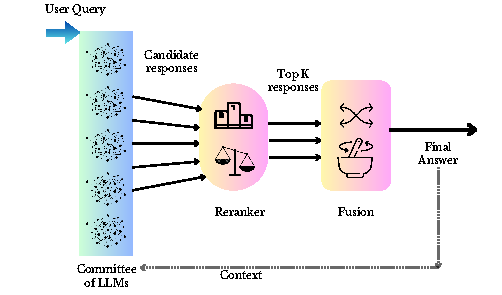
\includegraphics[width=1\linewidth]{figures/llm-blender.pdf}
    \caption{Overview of LLM Blender}
    \label{fig:llm-blender}
\end{figure}




\begin{figure}[h!] 
    \centering
    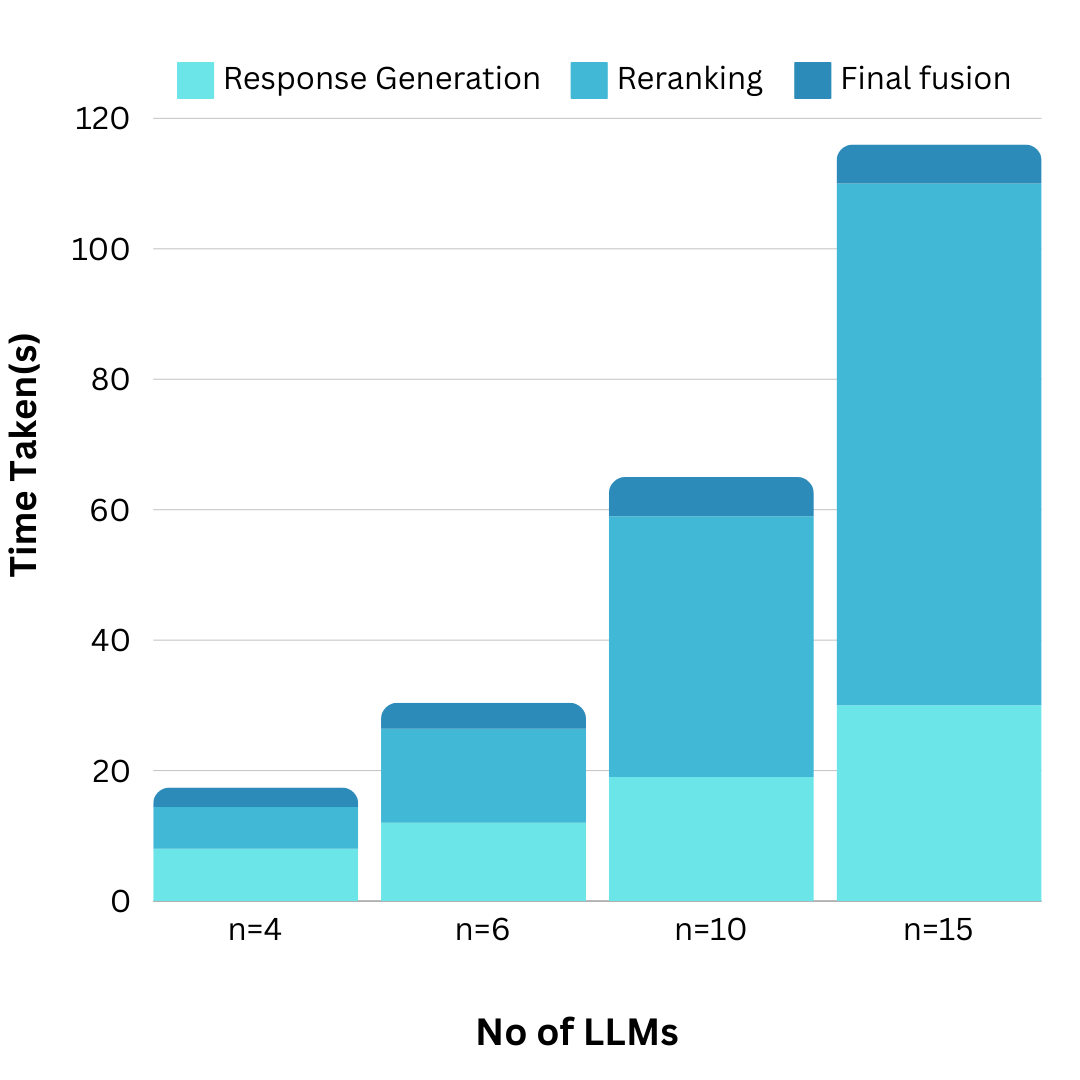
\includegraphics[width=0.5\linewidth]{figures/time-components.png}
    \caption{Time taken by different components of the LLMBlender system scales with the number of LLMs.}
    \label{fig:time-comp}
\end{figure}

\begin{figure}[h!] 
    \centering
    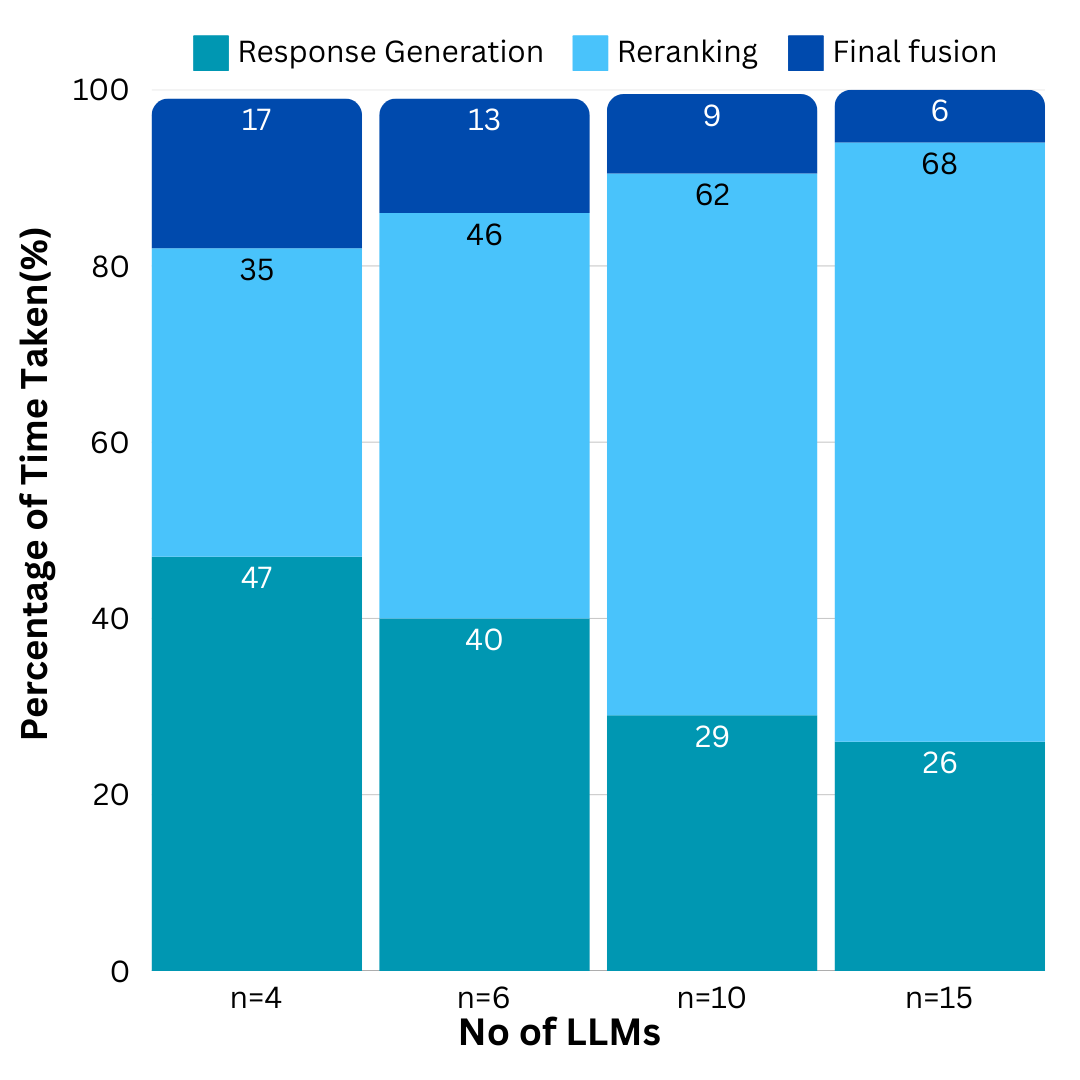
\includegraphics[width=0.5\linewidth]{figures/time-percentage.png}
    \caption{Ratio of time taken in blending by different components as the system scales with the number of LLMs.}
    \label{fig:scale}
\end{figure}

While there have been various studies examining the performance and latency of these frameworks, much of the existing research focuses on the overall effectiveness of ensembling without giving sufficient attention to the trade-offs between performance and latency. Current literature tends to treat reranking and fusion as static components, without delving into how tuning these mechanisms could improve system efficiency. There is a gap in the literature regarding comprehensive studies on how changes to reranking strategies or dynamic adjustments to K in fusion mechanisms could strike a better balance between high performance and low latency.



The aim of this paper is to fill this gap by providing an in-depth analysis of the performance-latency trade-offs in ensembling frameworks. Specifically, we explore different meta-ranking paradigms designed to reduce the frequency of reranking without causing a significant drop in performance. By adopting more efficient ranking strategies, we demonstrate that latency can be significantly reduced, making these frameworks more suitable for real-time applications. Additionally, we conduct a detailed study of the fusion mechanism, particularly focusing on how varying the value of K impacts both performance and latency. 



Using a cached ranking mechanism, we aim to achieve two benefits: (1) bypassing the reranker, which operates at \(O(N^2)\) complexity, thereby improving efficiency, and (2) narrowing response generation to the top-K selected LLMs based on cached rankings, eliminating the need to query all \(N\) LLMs. This approach significantly optimizes computational resources and response time.

\begin{figure}{0.8\linewidth}
    \centering
    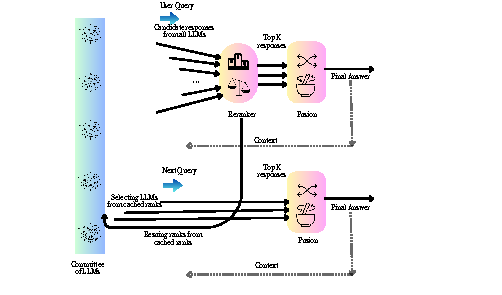
\includegraphics[width=1\linewidth]{figures/overview.pdf}
    \caption{Overview of the cached ranking mechanism}
    \label{fig:scale}
\end{figure}

Our experiments employ a committee of ten lightweight, open-source LLMs evaluated on two datasets: ConvQuestions and Atlas -conversation, both of which focus on conversational question answering. We use BERTScore \cite{zhang2020bertscoreevaluatingtextgeneration} a widely used metric for text generation  to measure the quality of responses. Our experiments show that there is often an optimal K beyond which adding more responses to the blend results in diminishing returns in terms of quality.

Our findings highlight two key insights: first, reducing the frequency of reranking, even in simple ways, leads to substantial latency reductions while maintaining strong performance. Second, the selection of an optimal K is critical for maximizing the effectiveness of the fusion mechanism, as blending too many responses can lead to a drop in quality.

In conclusion, our contributions demonstrate how ensembling frameworks can be optimized for better performance-latency trade-offs by adjusting reranking strategies and dynamically selecting K for response fusion. These findings have the potential to enhance the practical deployment of such frameworks, especially in real-time systems, by offering a balance between computational efficiency and high-quality output.

\section{Related Work}

Research on large language models (LLMs) indicate significant variability in performance across tasks, making the selection and optimization of LLMs an active area of study. Below, we list key advancements and their limitations.

Jiang et al. \cite{jiang-etal-2023-llm} show the distribution of the top-performing LLMs across 5,000 instructions. The results based on how frequently each LLM ranks first in different instances shows that the best LLM for any given task can vary significantly, depending on the topic, type of question and complexity of query.

Weizhou Shen et. al. \cite{shen2024smallllmsweaktool} claim that traditional approaches that rely on a single LLM for multiple capabilities often face performance limitations, particularly with smaller models. To address this, they propose a modular framework that decomposes tasks into a planner, caller, and summarizer, each handled by separate LLMs specialized for their respective roles. This framework, trained through a two-stage process, allows for easier updates, the use of smaller models, and achieves superior performance compared to single-LLM approaches, as demonstrated in various tool-use benchmarks.

Lu et.al. in their study of ``Blending Is All You Need''\cite{lu2024blendingneedcheaperbetter} investigate whether smaller models can collaboratively achieve performance comparable to or exceeding that of a single large model like ChatGPT, which has over 175 billion parameters. By integrating multiple smaller chat AIs (blending) the research demonstrates that combining just three moderate-sized models (6B/13B parameters) can match or surpass the performance of alone larger counterparts. Empirical results from A/B testing on the Chai research platform over thirty days highlight the effectiveness of the blending strategy in enhancing chat AI performance while minimizing computational resource requirements.

To combine the strengths of multiple large language models (LLMs), we incorporate frameworks consisting of multile smaller LLMs. These frameworks aim to combine the diverse capabilities of various LLMs by selecting an optimal subset of models based on a given query and then blending the responses from the selected models. Such an approach can lead to higher-quality responses as it benefits from the complementary strengths of the different models. Such ensembling framework aim to give a more consistent performance.

One prominent example of this is LLMBlender \cite{jiang-etal-2023-llm}, which consists of two main components: the first is a mechanism for selecting the optimal subset of LLMs based on the nature of the query, and the second is a fusion mechanism to combine the responses generated by the selected models.

There are two primary approaches to ensemble large language models (LLMs): selection-based and generation-based methods. Selection-based methods involve comparing the candidates within the set \( Y \) and selecting the top-ranked candidate as the final output \( \hat{y} \), which implies that \( \hat{y} \in Y \). Due to the nature of selection and the constrained solution space, the performance of selection-based methods is inherently limited by the \( N \) candidates being considered. In contrast, generation-based methods focus on fusing \( K \) candidates (where \( 1 < K \leq N \)) from \( Y \) to produce a novel response as the final output \( \hat{y} \).

But they face a significant challange in deployement. The selection process typically involves brute-force reranking of all available pair to determine the optimal subset, which is computationally expensive and time-consuming. This makes these frameworks difficult to deploy in real-time systems where quick response times are critical, such as in interactive question-answering systems. Furthermore, most ensembling frameworks employ a fixed value of K, meaning they always blend the top K responses, regardless of whether blending more or fewer responses might yield better or faster results. Works like selectLLM addresses this by selecting a smaller subset of LLMs based on query then following a fixed policy to combine the best responses.

Open-source LLMs display a range of strengths and weaknesses due to differences in their data, architectures, and hyperparameters, making them complementary. 
Jiang et al. \cite{jiang-etal-2023-llm} demonstrate that the performance of LLM for any given task can vary significantly, implying that the best suited LLM among a commitee of LLM for a common task vary depending on the topic, type of input and complexity of query. 

To overcome the challenges posed by the limited knowledge of LLMs, researchers have developed various techniques to enhance their capabilities. Retrieval-Augmented Generation (RAG) \cite{lewis2020retrieval} is one such approach, wherein the models responses are informed by external knowledge repository. However, the accuracy of RAG still heavily depends on the effectiveness of the underlying encoder and the fuser models to have sound understanding of the queries. 

Another promising approach is LLMRoute \cite{srivatsa2024harnessing, deepseekai2024deepseekv3technicalreport}
, which seeks to harness the combined potential of multiple expert Feedforwrds together by dynamically routing queries to the most suitable expert. While LLMRoute improves performance by routing the queries to specialized experts, it is limited by its design of selecting only one expert at a time. This approach is suboptimal for handling interdisciplinary queries that require synthesizing knowledge from multiple LLMs simultaneously, thereby limiting its effectiveness in such scenarios.


Han Yang developed a novel ensemble learning pipeline using state-of-the-art LLMs to improve accuracy and reliability in diverse medical question-answering (QA) tasks. This approach focuses on enhancing performance across three medical QA datasets: PubMedQA, MedQA-USMLE, and MedMCQA. The study aims to explore efficient methods for deploying LLM technologies in medical QA applications.

Shekhar et al. discusses about the quality vs cost tradeoff in LLMs, highlighting the difficulty in estimating LLM performance and costs upfront, noting that current methods rely on runtime evaluations, which can increase costs and latency and not a practical score, and introduce a quality metric to align with human perceptions of text quality.

In-context learning (ICL) enables LLMs to adapt quickly to diverse tasks but is highly sensitive to factors like prompt design and demonstration ordering. Demonstration selection strategies are categorized into task-specific scorers with external supervision and task-agnostic contrast-based measures derived from LLM predictions. Approaches like Sentence-BERT, k-Nearest Neighbors, contrastive scoring, and Determinantal Point Processes (DPPs) have been used to optimize demonstration selection for improved ICL performance.\cite{izacard2022unsuperviseddenseinformationretrieval}


With the growing diversity of multi-LLM tasks and variable pricing structures, selecting the optimal LLM selection configuration has become increasingly important. The C2MAB-V framework \cite{dai2024costeffectiveonlinemultillmselection} tackles this by using a Cost-effective Combinatorial Multi-armed Bandit approach that optimizes LLM selection across different reward models, balancing performance and cost. It addresses the multi-LLM selection challenge through an exploration-exploitation trade-off, online feedback, and integer programming techniques, proving effective in both theory and practice across multiple application scenarios. On the same problem, Yu Xia  propose TI-UCB \cite{xia2024llmplayconvergenceawareonline}, a time-increasing bandit algorithm that predicts performance improvements from finetuning and uses change detection to capture convergence points, achieving lower regret and improved model selection efficiency.

\section{Our Work}

\subsection{Objective}
The primary objective of this work is to study the trade-offs between latency and performance in an LLM ensemble framework, with the goal of designing a lightweight, easily deployable system. Specifically, we analyze the impact of ranking on fusion, measuring the speedup and responsiveness gains that may come at the cost of reduced output quality when skipping ranks.

Given an input \( \mathcal{D}_x \) and a set of \( N \) LLMs \( \{ M_1, M_2, \ldots, M_N \} \), we generate \( N \) candidate outputs by processing \( \mathcal{D}_x \) through each model. The candidate set is denoted as \( Y = \{ y_1, y_2, \ldots, y_N \} \), where each \( y_i \) is the output generated by model \( M_i \). In the training phase, a ground truth output \( y \) is assumed to exist, though it remains hidden during evaluation in the test phase.

Our objective is to rigorously study the trade-off between quality and efficiency in an ensemble framework for large language models (LLMs). Specifically, we aim to analyze the impact of avoiding ranking on both the quality of the final output and the speedup in response time. Let \( Q(y, \hat{y}; x) \) denote the quality function that measures the similarity between the ground truth output \( y \) and the predicted output \( \hat{y} \) for a given input \( x \). Additionally, let \( T(x) \) denote the time taken to generate the output for input \( x \).

We aim to quantify the trade-offs when the ranking process is skipped. To this end, we introduce a binary decision variable \( r \in \{0, 1\} \), where \( r = 1 \) indicates that ranking is applied, and \( r = 0 \) indicates that ranking is avoided. Our objective is to study how the absence of ranking (i.e., \( r = 0 \)) affects the quality \( Q \) and time \( T \). Formally, for a test set \( D_{\text{test}} = \{ (x^{(i)}, y^{(i)}) \} \), we aim to study the degradation in quality \( \Delta Q(r) \) and the speedup \( \Delta T(r) \) as functions of \( r \), where:

\[
\Delta Q(r) = \sum_{i} \left( Q(y^{(i)}, \hat{y}^{(i)}; x^{(i)}, r = 1) - Q(y^{(i)}, \hat{y}^{(i)}; x^{(i)}, r = 0) \right)
\]

\[
\Delta T(r) = \sum_{i} \left( T(x^{(i)}, r = 0) - T(x^{(i)}, r = 1) \right)
\]

Additionally, we aim to investigate the optimal number of models \( K \) to fuse in the ensemble process. We hypothesize that the number of models \( K \) affects both the performance and the time complexity of the ensemble method. To capture this, we study the variation in quality \( Q \) as a function of \( K \), both with and without ranking. Formally, we aim to analyze the following:

\[
Q(K, r) = \sum_{i} Q(y^{(i)}, \hat{y}^{(i)}(K, r); x^{(i)})
\]

where \( \hat{y}^{(i)}(K, r) \) is the output produced by fusing the top \( K \) models (or \( K \) randomly selected models if ranking is avoided, i.e., \( r = 0 \)) for input \( x^{(i)} \).

Our goal is to determine the optimal value of \( K \) that maximizes quality while minimizing time, both with and without ranking, thereby quantifying the trade-offs in performance and latency when the ranking process is skipped.

\subsection{Problem Setup}


We use the \textit{LLM-BLENDER} for our experiments, a framework designed to improve performance by blending the outputs of multiple large language models (LLMs). LLM-BLENDER is composed of two core components: \textit{PAIRRANKER} and \textit{GENFUSER}. 

Let the set of candidate outputs from \( N \) LLMs for an input \( x \) be denoted as \( Y = \{ y_1, y_2, \ldots, y_N \} \), where \( y_i \) represents the output of model \( M_i \) for the same input. The \textit{PAIRRANKER} module ranks these outputs using a scoring function \( S(y_i, x) \), where \( S: Y \times \mathcal{X} \to \mathbb{R} \) assesses the quality or relevance of candidate \( y_i \) with respect to the input \( x \).

\begin{algorithm}
\caption{Pairwise Scoring and Aggregation with MaxLogits}
\label{alg:combined_algorithm}
\begin{algorithmic}[1]

\Require Set of candidates $Y = \{y_1, y_2, \dots, y_N\}$, scoring function $f(y_i, y_j)$
\Ensure Scores $s_i$ for each candidate $y_i$

\Statex
\Function{MatrixConstruction}{$Y$, $f$} \Comment{Routine 1}
    \State Initialize $M \gets 0^{N \times N}$
    \For{$i \gets 1$ to $N$}
        \For{$j \gets 1$ to $N$}
            \If{$i \neq j$}
                \State $M_{ij} \gets f(y_i, y_j)$ \Comment{Compute confidence that $y_i$ is better than $y_j$}
            \Else
                \State $M_{ij} \gets 0$ \Comment{No self-comparison}
            \EndIf
        \EndFor
    \EndFor
    
    \Return $M$
\EndFunction

\Statex
\Function{MaxLogitsAggregation}{$M$} \Comment{Routine 2}
    \For{$i \gets 1$ to $N$}
        \State $M^*_i \gets$ $i$-th row of $M$
        \State $M_i^* \gets$ $i$-th column of $M$
        \State $s_i \gets \sum (M^*_i - M_i^*)$
    \EndFor
    
    \Return $s_1, s_2, \dots, s_N$
\EndFunction

\Statex
\State $M \gets$ \Call{MatrixConstruction}{$Y$, $f$} \Comment{Call Routine 1}
\State $s_1, s_2, \dots, s_N \gets$ \Call{MaxLogitsAggregation}{$M$} \Comment{Call Routine 2}

\end{algorithmic}
\end{algorithm}

In LLM-BLENDER, \textit{PAIRRANKER} is implemented using a DeBERTa-v3-large encoder model, pre-trained with annotated ranks. The output is a ranked list of the top \( K \) outputs \( Y_{\text{top}} = \{ y_{\sigma(1)}, y_{\sigma(2)}, \ldots, y_{\sigma(K)} \} \), where \( \sigma \) is a permutation function ordering the outputs according to their scores:

\[
S(y_{\sigma(1)}, x) \geq S(y_{\sigma(2)}, x) \geq \cdots \geq S(y_{\sigma(N)}, x)
\]




After selecting the top \( K \) ranked outputs \( Y_{\text{top}} \), the \textit{GENFUSER} module fuses these outputs to produce a final output \( \hat{y} \). Formally, the fusion function \( F \) takes the top-ranked outputs as input and generates the final output as:

\[
\hat{y} = F(y_{\sigma(1)}, y_{\sigma(2)}, \ldots, y_{\sigma(K)})
\]



The ranking mechanism employs a pairwise comparison approach to score and rank candidate responses. First, a pairwise score matrix \(M\) is constructed, where each entry \(M_{ij}\) represents the confidence that candidate \(y_i\) is better than \(y_j\), using a scoring function \(f(y_i, y_j)\). Next, the aggregation method computes a confidence score \(s_i\) for each candidate by summing the differences between the respective row and column entries of \(M\), reflecting \(y_i\)'s relative strength against all others. This approach balances precision and efficiency, enabling robust ranking while maintaining scalability for larger candidate sets.


The fusion function \( F \) uses a generation process to synthesize a new response using the knowledge in individual LLM reponse. In LLM-BLENDER, \textit{GENFUSER} is implemented using a fine-tuned Flan-T5-xl model (3 billion parameters) in a sequence-to-sequence (seq2seq) setting.

The objective of \textit{GENFUSER} during training is to maximize the similarity between the final fused response \( \hat{y} \) and the ground truth summary \( y \):

\[
\hat{y} = \arg\min_{\hat{y}} Dist(y, \hat{y}; x)
\]

By using both the ranking produced by PAIRRANKER and the fusion mechanism in GENFUSER, LLM-BLENDER outperform any single LLM in generating high-quality outputs.


\subsection{Dataset and Models}
To evaluate the performance of our ensemble framework, we conduct experiments on two prominent datasets for Conversational Question Answering (CQA): \text{ConvQuestions} and \text{Atlas-conversation}. These datasets represent different styles of conversational interactions and question complexities, allowing us to assess the robustness of our approach across diverse scenarios.

\text{ConvQuestions Dataset} is a realistic benchmark for conversational question answering compiled by 70 Master crowdworkers on Amazon Mechanical Turk, who designed conversations within five domains: Books, Movies, Soccer, Music, and TV Series. This dataset is notable for featuring a wide variety of challenging question types, each based on entities from Wikidata, ensuring that answers are grounded in a structured, consistent knowledge graph. All questions in a conversation are posed by the same annotator, who also provided gold-standard answers. The focus on natural language and the allowance of diverse question types makes ConvQuestions particularly challenging.


The \text{Atlas-conversation} datasetcontains a large number of conversational examples with diverse question types and styles, offering a rich testing ground for CQA systems. The dataset features a hierarchical structure of 41 main categories, with subcategories

In our experiments, we employ a diverse selection of state-of-the-art open-source large language models (LLMs) to explore the effectiveness of our ensemble framework. The models used in this study include both high-performance and lightweight variants, allowing us to evaluate the trade-offs between model complexity, latency, and performance.

The LLMs used in our evaluation are as follows:

\begin{itemize} \item \textbf{Mistral}: A cutting-edge LLM known for its superior performance across various natural language processing tasks. \item \textbf{LLaMA 3.1}: A highly efficient LLM designed to achieve strong results in language generation and understanding. \item \textbf{Gemma:2B}: A lightweight, 2-billion parameter model optimized for fast, responsive conversational tasks. \item \textbf{Phi3}: A high-capacity LLM built for handling more complex linguistic and reasoning challenges. \item \textbf{Qwen:4B}: A robust 4-billion parameter model with enhanced contextual understanding, especially in dialogue systems. \item \textbf{Phi}: Another variant of the Phi model family, specialized for knowledge retrieval and reasoning. \item \textbf{TinyDolphin}: A compact, fast model designed for low-latency text generation in real-time environments. \item \textbf{DeepSeek-LLM}: Known for its strong generalization, particularly useful for knowledge-based question answering. \item \textbf{StableLM2}: A highly stable LLM optimized for consistent conversational performance. \item \textbf{Dog/Arcee-Lite}: A lightweight model built for fast and scalable inference with a focus on minimal latency. \item \textbf{Sunwon/Tiny}: A small, efficient LLM aimed at quick text generation tasks with minimal resource consumption. \item \textbf{OpenChat}: Designed specifically for interactive dialogue, this model excels in human-like conversational capabilities. \item \textbf{Hermes3}: A powerful LLM with advanced reasoning and natural language understanding capabilities. \item \textbf{StableLM-Zephyr}: An LLM optimized for high-speed text generation without compromising quality. \item \textbf{MistralLite}: A lightweight version of Mistral, offering a balance between performance and computational efficiency. \end{itemize}

\section{Experiment}
\subsection{Ranking of LLM Responses}

In this experiment, we passed questions from both datasets—ConvQuestions and Atlas-Conversation—through the LLM-BLENDER framework. For each input, the framework generated responses from all participating large language models (LLMs) and subsequently ranked these responses using the PAIRRANKER module. The purpose of this experiment was to observe the distribution of rankings across the LLMs and determine which models consistently ranked higher and which did not.

\begin{figure}[htbp]
    \centering
    \subfigure[ConvQuestions]{
        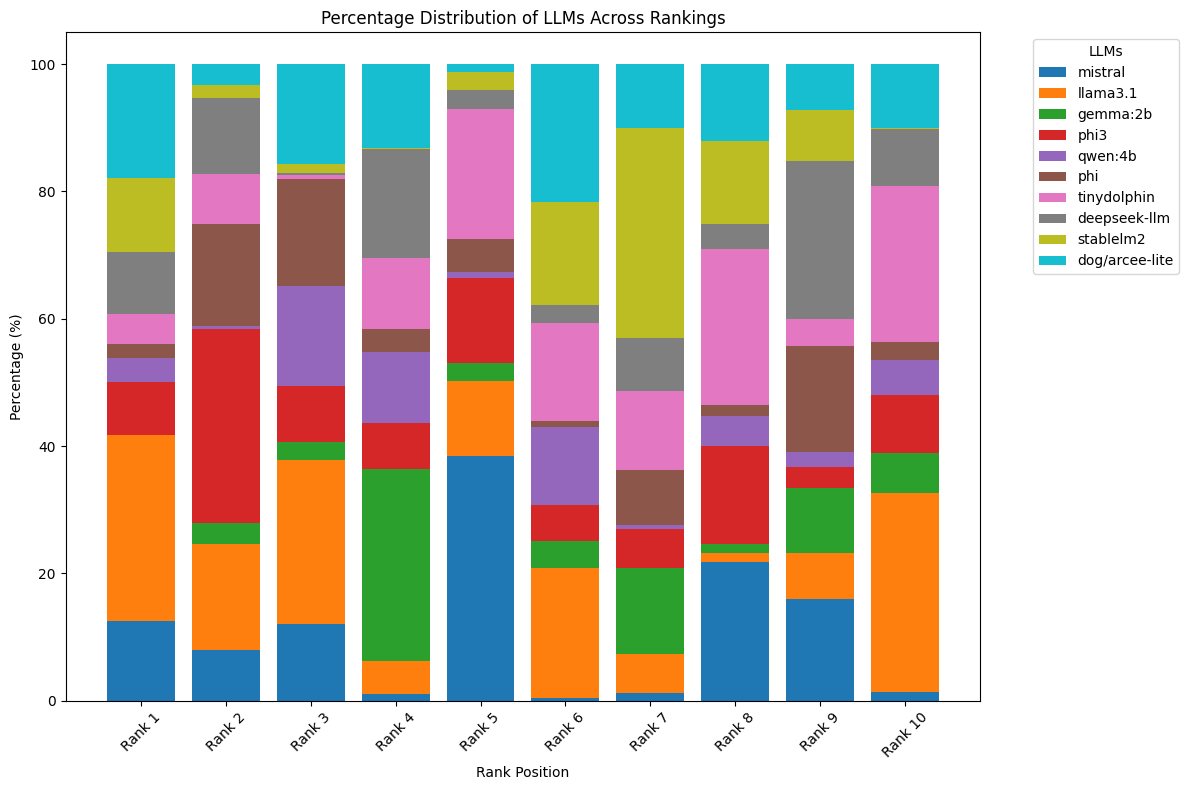
\includegraphics[width=1\linewidth]{figures/LLMRanks.png}
        \label{fig:convquestions-ranking}
    }
    \hspace{0.05\linewidth} % Optional horizontal space between figures
    \subfigure[Atlas]{
        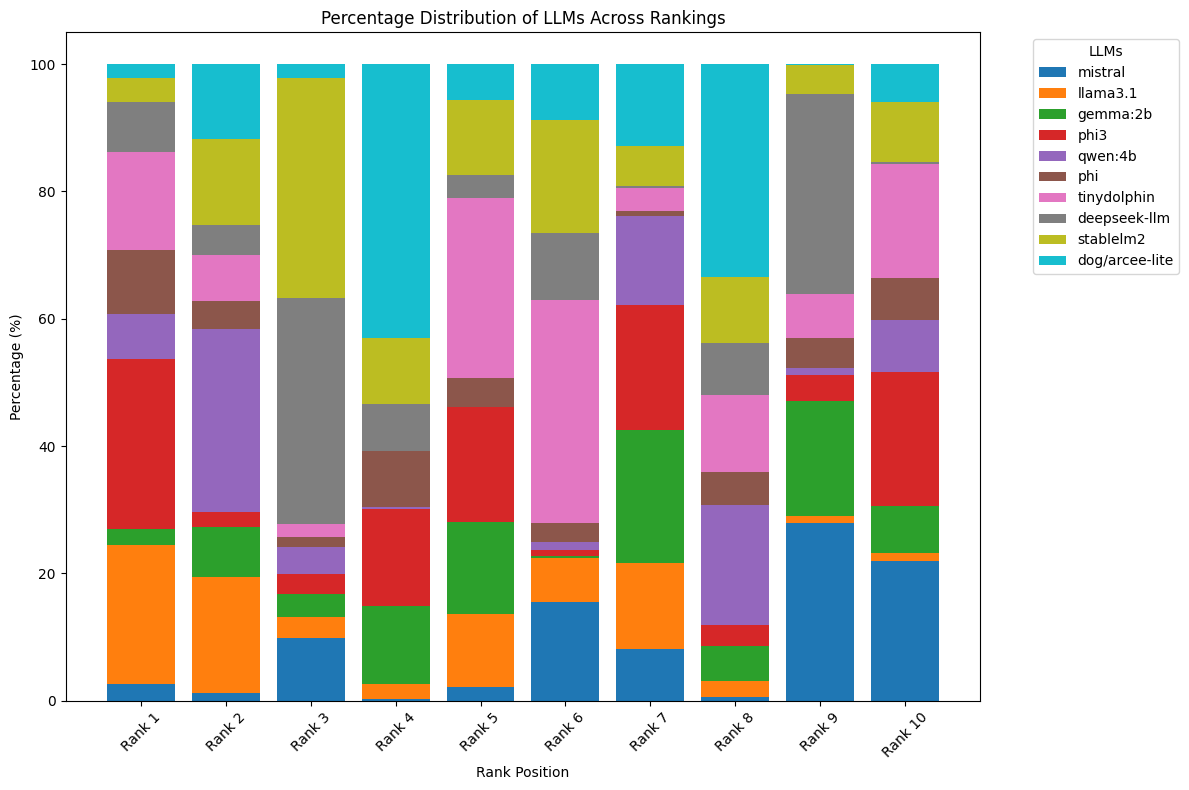
\includegraphics[width=1\linewidth]{figures/LLMRanks2.png}
        \label{fig:atlas-conversation-ranking}
    }
    \caption{Distribution of rankings across LLMs for both datasets. Different bars represent different ranks from 1 to 10 as left to right. Different color pieces represeent the different LLMs. The length of the colored pieces represent the percentage of times of getting that particular rank by the LLM-Blender}
    \label{fig:ranking-distribution}
\end{figure}





Our observations revealed interesting patterns. Within the context of a single conversation, certain LLMs consistently outperformed others, establishing themselves as more effective for that particular topic. These LLMs, which we term "high-performing LLMs," tend to dominate the rankings and are frequently selected for response generation. On the contrary, some LLMs, which we refer to as "low-performing LLMs," consistently ranked lower in the same conversation, indicating they were less suited to that specific topic or question type.

However, as the conversation shifts to a different domain or topic, we observed a shift in rankings. LLMs that ranked lower in the previous conversation suddenly performed better in the new context, replacing the previously dominant models. This indicates that the performance of each LLM is highly context-dependent, and no single LLM consistently outperformed others across all conversations.

Interestingly, across the full set of conversations, all LLMs were ranked in the top positions at least once for some topics. This variability made it challenging to identify and eliminate "low-performing" LLMs across all conversations, as an LLM that performed poorly in one domain could excel in another. Therefore, our findings suggest that while certain LLMs may appear to underperform in specific contexts, they are valuable for different types of conversations, and eliminating them based on a single topic would be suboptimal.

This ranking experiment highlights the necessity of employing dynamic ensembling techniques, as the optimal LLM varies depending on the conversation's subject matter. It also underscores the importance of considering a diverse set of LLMs to ensure coverage across various topics and domains.

\subsection{Strategies to Avoid Ranking: Quality vs Latency}

We conducted experiments to study the trade-offs between response quality and speedup when avoiding full ranking. Below, we describe the different strategies that were explored, comparing them with the baseline full ranking approach.

\subsubsection{1. Full Ranking (Baseline)}
This strategy serves as the baseline. For every conversation, we compute pairwise comparisons between all \( N \) LLMs, resulting in \( \binom{N}{2} \) comparisons. This exhaustive ranking allows us to choose the best-performing LLMs based on complete information.

\begin{itemize}
    \item \textbf{Quality}: Highest, as all LLMs are fully compared in each conversation.
    \item \textbf{Latency}: Highest, since the number of comparisons scales quadratically with the number of LLMs.
\end{itemize}

\begin{algorithm}[H]
\caption{Full Ranking Baseline}
\label{alg:full_ranking}
\begin{algorithmic}[1]
\Require Set of LLMs $\mathcal{L} = \{\text{LLM}_1, \text{LLM}_2, \dots, \text{LLM}_N\}$, user query $q$
\Ensure Final fused answer $a_{\text{final}}$
\State Initialize empty list of responses $\mathcal{R} \gets []$
\For{each $\text{LLM}_i \in \mathcal{L}$}
    \State $\text{response}_i \gets \text{LLM}_i(q)$ \Comment{Generate response for the query}
    \State Append $\text{response}_i$ to $\mathcal{R}$
\EndFor
\State Compute pairwise score matrix $M \in \mathbb{R}^{N \times N}$, where $M_{ij} \gets f(\text{response}_i, \text{response}_j)$
\State Rank all LLMs based on scores derived from $M$ \Comment{Full pairwise ranking}
\State Select top $k$ LLMs $\mathcal{L}_{\text{top}} \subseteq \mathcal{L}$ based on the ranking
\State Aggregate responses from $\mathcal{L}_{\text{top}}$ to produce final fused answer $a_{\text{final}}$
\Return $a_{\text{final}}$
\end{algorithmic}
\end{algorithm}


% \subsubsection{2. Harsh Elimination}
% In this approach, we perform full ranking for the first five conversations. Afterward, the bottom-performing LLMs are permanently eliminated for all upcoming conversations. 

% \begin{itemize}
%     \item \textbf{Quality}: Lowest, as eliminating certain LLMs early reduces the pool of candidates, and some LLMs may excel in later conversations but do not get the chance.
%     \item \textbf{Latency}: Best, with significant speedup due to reduced ranking computations after the initial phase.
% \end{itemize}

\subsubsection{2. Fixed-Interval Elimination}
Here, we rank all questions within the first conversation to identify top and bottom-performing LLMs. The bottom \( \frac{N}{2} \) LLMs are excluded for the next 10 conversations. Afterward, all LLMs rejoin, and the process repeats.

\begin{itemize}
    \item \textbf{Quality}: Moderate, with some degradation as eliminated LLMs may have contributed in subsequent conversations. However, the reintroduction after 10 conversations mitigates the quality drop.
    \item \textbf{Latency}: Good, with substantial speedup due to the temporary exclusion of half of the LLMs for an extended period.
\end{itemize}




\subsubsection{3. Dynamic Conversation-Specific Elimination}
For each conversation, we rank only the first \( \lceil \frac{q}{2} \rceil \) questions (where \( q \) is the number of questions in the conversation) to identify top and low-performing LLMs. The bottom \( N - \lceil \frac{N}{2} \rceil \) LLMs are eliminated for the next question within the same conversation. All LLMs rejoin at the start of each new conversation.

\begin{itemize}
    \item \textbf{Quality}: Near-optimal, closely approximating the full ranking strategy, as eliminations only affect part of each conversation. All LLMs rejoin after each conversation.
    \item \textbf{Latency}: Excellent, with up to 60\% reduction in latency. This strategy maintains a good balance between quality and computational efficiency.
\end{itemize}




\subsubsection{4. Combining Interval based and Conversation Specific - Alternate ranking}
For each query, we rank once, then in the next query in the same conversation we do not rank. All LLMs rejoin at the start of each new conversation.

\begin{itemize}
    \item \textbf{Quality}: Near-optimal, best approximating the full ranking strategy.
    \item \textbf{Latency}: Excellent, with up to 25\% reduction in latency. This strategy maintains a good quality.
\end{itemize}

\begin{algorithm}
\caption{Algorithms using Rank Caching Policies}
\label{alg:llm_selection_algorithms}

\vspace{1em}

\textbf{Policy 1: Fixed-Interval Elimination}
\begin{algorithmic}[1]
\Require Set of LLMs $\mathcal{L}$, set of queries $\mathcal{Q}$, elimination interval $I$, scoring function $f$
\Ensure Final answers $\mathcal{A} = \{a_1, a_2, \dots, a_{|\mathcal{Q}|}\}$
\State $\mathcal{L}_{\text{active}} \gets \mathcal{L}$
\For{$t \gets 1$ to $|\mathcal{Q}|$}
    \State Generate responses $\mathcal{R} = \{\text{LLM}_i(q_t) \mid \text{LLM}_i \in \mathcal{L}_{\text{active}}\}$
    \If{$t \mod I = 1$ and $t > 1$}
        \State $\mathcal{L}_{\text{active}} \gets \mathcal{L}$
    \ElsIf{$t \mod I = 0$}
        \State Compute pairwise score matrix $M$
        , where $M_{ij} \gets f(\text{response}_i, \text{response}_j)$
        \State Rank LLMs in $\mathcal{L}_{\text{active}}$ based on $M$
        \State $\mathcal{L}_{\text{active}} \gets$ Top $\lceil \frac{N}{2} \rceil$ LLMs
    \EndIf
    \State Aggregate responses from $\mathcal{L}_{\text{active}}$ to produce $a_t$
    \State Append $a_t$ to $\mathcal{A}$
\EndFor
\Return $\mathcal{A}$
\end{algorithmic}

\textbf{Policy 2: Conversation-Specific Elimination}
\label{alg:dynamic_elimination}
\begin{algorithmic}[1]
\Require Set of LLMs $\mathcal{L}$, conversations $\mathcal{C}$, scoring function $f$
\Ensure Final answers $\mathcal{A} = \{a_{c,t}\}$ for each conversation $c$ and question $t$
\For{each conversation $c \in \mathcal{C}$}
    \State $\mathcal{L}_{\text{active}} \gets \mathcal{L}$ \Comment{Reinitialize all LLMs for each conversation}
    \State Get questions $\mathcal{Q}_c = \{q_{c,1}, q_{c,2}, \dots, q_{c,|\mathcal{Q}_c|}\}$ for conversation $c$
    \State Let $T_{\text{rank}} \gets \lceil \frac{|\mathcal{Q}_c|}{2} \rceil$ \Comment{Number of questions for ranking}
    \For{$t \gets 1$ to $|\mathcal{Q}_c|$}
        \State Initialize empty list of responses $\mathcal{R} \gets []$
        \For{each $\text{LLM}_i \in \mathcal{L}_{\text{active}}$}
            \State $\text{response}_i \gets \text{LLM}_i(q_{c,t})$ \Comment{Generate response for question $t$}
            \State Append $\text{response}_i$ to $\mathcal{R}$
        \EndFor
        \If{$t \leq T_{\text{rank}}$} \Comment{Perform ranking on the first $\lceil \frac{|\mathcal{Q}_c|}{2} \rceil$ questions}
            \State Compute pairwise score matrix $M \in \mathbb{R}^{|\mathcal{L}_{\text{active}}| \times |\mathcal{L}_{\text{active}}|}$
            \State Rank LLMs in $\mathcal{L}_{\text{active}}$ based on scores from $M$
            \State Select top $\lceil \frac{N}{2} \rceil$ LLMs from $\mathcal{L}_{\text{active}}$
            \State $\mathcal{L}_{\text{active}} \gets$ Selected top $\lceil \frac{N}{2} \rceil$ LLMs
        \EndIf
        \State Aggregate responses from $\mathcal{L}_{\text{active}}$ to produce final fused answer $a_{c,t}$
        \State Append $a_{c,t}$ to $\mathcal{A}$
    \EndFor
\EndFor
\Return $\mathcal{A}$
\end{algorithmic}

\end{algorithm}

\begin{algorithm}
\textbf{Policy 3: Alternating Ranks}
\begin{algorithmic}[1]
\Require Set of LLMs $\mathcal{L}$, set of conversations $\mathcal{C}$, scoring function $f$
\Ensure Final answers $\mathcal{A} = \{a_{c,t}\}$ for each conversation $c$ and query $t$
\For{each conversation $c \in \mathcal{C}$}
    \State $\mathcal{L}_{\text{active}} \gets \mathcal{L}$
    \For{$t \gets 1$ to $|\mathcal{Q}_c|$}
        \State Generate responses $\mathcal{R} = \{\text{LLM}_i(q_{c,t}) \mid \text{LLM}_i \in \mathcal{L}_{\text{active}}\}$
        \If{$t \mod 2 = 1$}
            \State Compute pairwise score matrix $M$
            \State Rank LLMs in $\mathcal{L}_{\text{active}}$ based on $M$
            \State $\mathcal{L}_{\text{active}} \gets$ Top $\lceil \frac{N}{2} \rceil$ LLMs
        \EndIf
        \State Aggregate responses from $\mathcal{L}_{\text{active}}$ to produce $a_{c,t}$
        \State Append $a_{c,t}$ to $\mathcal{A}$
    \EndFor
\EndFor
\Return $\mathcal{A}$
\end{algorithmic}
\end{algorithm}





\begin{figure}
    \centering
    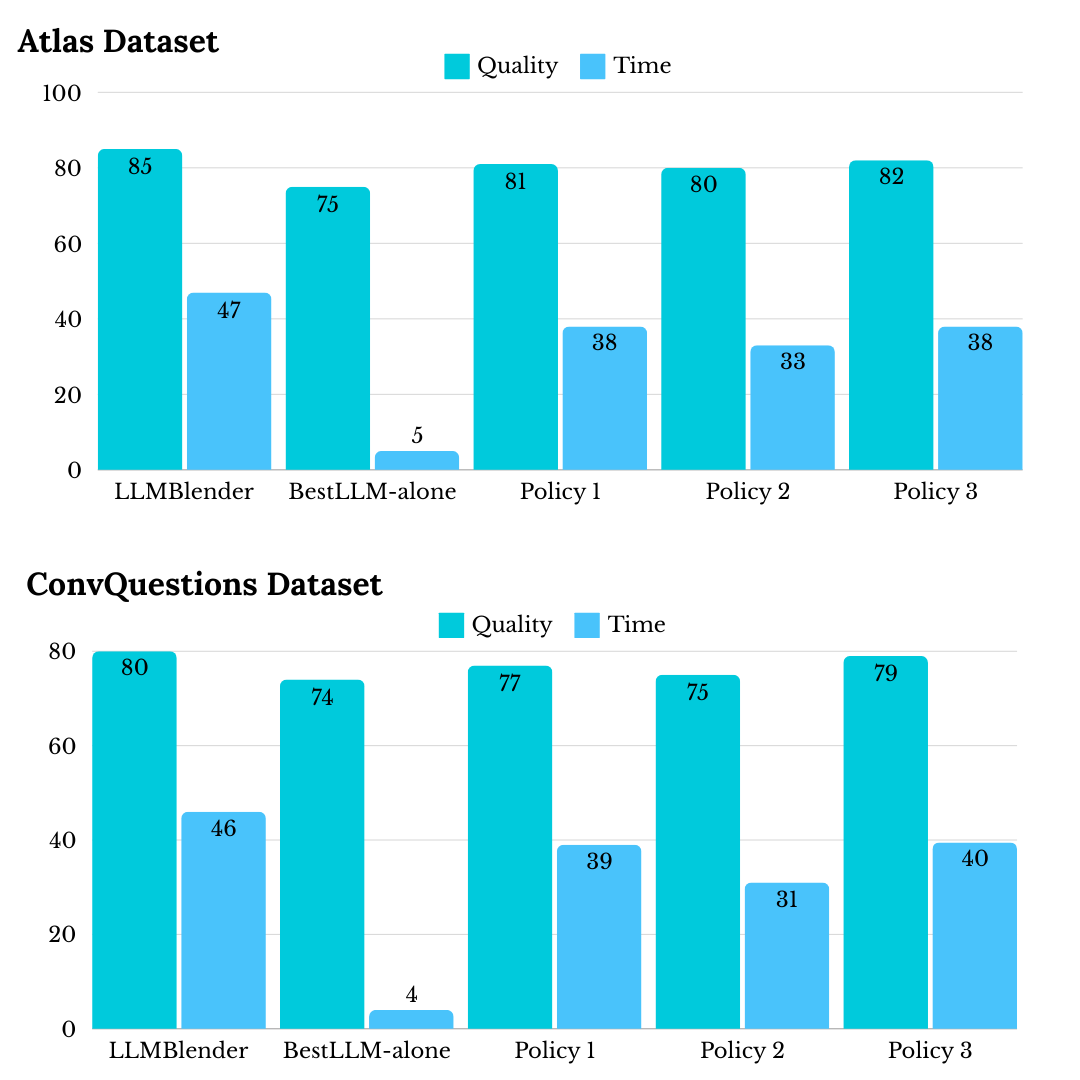
\includegraphics[width=0.7\linewidth]{figures/time-quality.png}
    \caption{Trade-offs between response quality and speedup when avoiding full ranking on ConvQuestions Dataset. LLMBlender (first from left) represents the full-ranking. BestLLM-alone (second from left) represents the best performing LLM taken alone}
    \label{fig:enter-label}
\end{figure}

% \begin{figure}
%     \centering
%     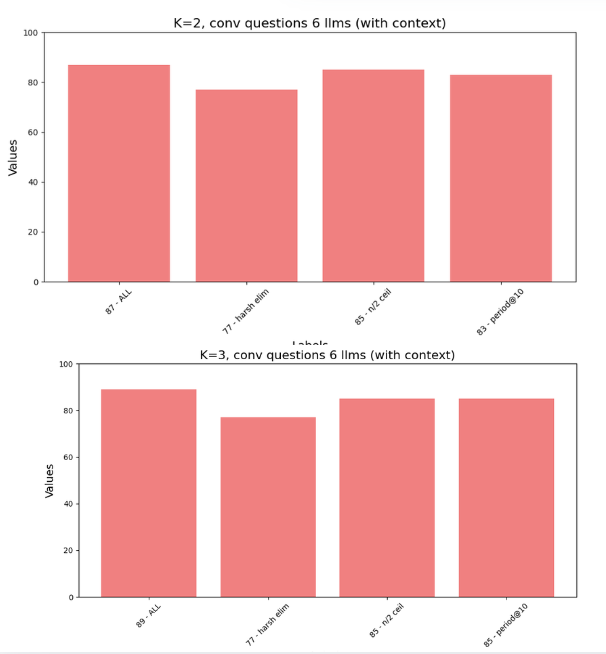
\includegraphics[width=0.7\linewidth]{figures/image3.png}
%     \caption{Experiments to study the trade-offs between response quality and speedup when avoiding full ranking on Atlas Dataset}
%     \label{fig:enter-label}
% \end{figure}

\subsubsection{Observations}
\begin{figure}
    \centering
    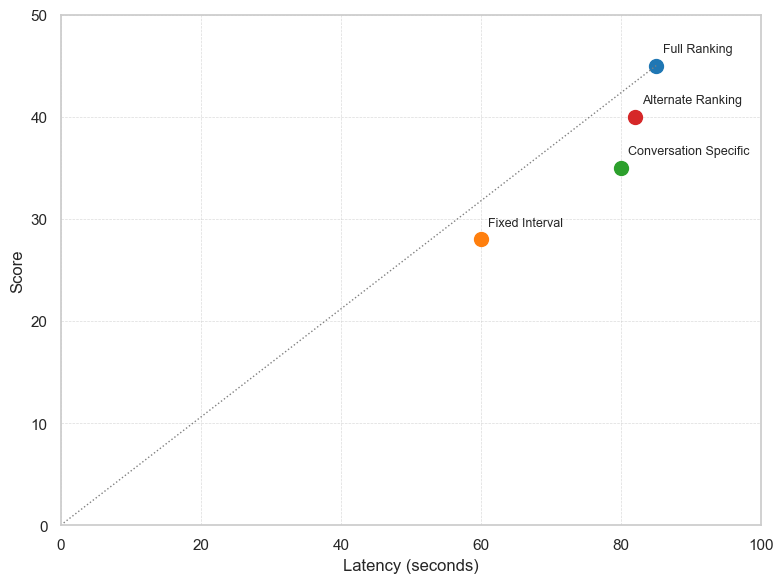
\includegraphics[width=0.75\linewidth]{figures/tradeoff.png}
    \caption{Score vs. Latency Tradeoff Across Ranking Strategies on ConvQuestions Dataset}
    \label{fig:tradeff}
\end{figure}

\textbf{Score vs. Latency Tradeoff Across Ranking Strategies}: Figure \ref{fig:tradeff} illustrates the tradeoff between latency (in seconds) and overall performance score across four ranking strategies: Full Ranking, Fixed Interval, Conversation Specific, and Alternate Ranking. The X-axis denotes latency, while the Y-axis shows performance score. Each strategy’s position indicates its balance between computational efficiency and ranking accuracy, with Full Ranking maximizing accuracy but incurring higher latency, while Fixed Interval significantly reduces latency at a modest cost in performance. 

\begin{itemize}
    \item \textbf{Full Ranking} provides the highest output quality but incurs the highest latency.
    % \item \textbf{Harsh Elimination} yields the best speedup but results in a substantial loss in quality due to the permanent elimination of LLMs.
    \item \textbf{Fixed-Interval Elimination} offers a good balance of speedup and moderate quality degradation, as LLMs are periodically reintroduced.
    \item \textbf{Dynamic Question-Specific Elimination} is the most effective strategy, achieving nearly the same quality as full ranking while significantly reducing computational time.
\end{itemize}

\begin{table}
    \centering
    \caption{Latency Comparison for Different Strategies}
    \label{tab:latency_comparison}
    \begin{tabular}{@{}lc@{}}
        \toprule
        \textbf{Strategy}               & \textbf{Latency (ms)} \\ \midrule
        Policy 1                        & 76363.6                \\
        Policy 2                        & 16800.3                \\
        Policy 3                        & 90033.9                 \\
        Full Ranking                    & 120004.5               \\ \bottomrule
    \end{tabular}
\end{table}

These experiments show us that while avoiding full ranking can significantly reduce latency, the optimal strategy depends on the trade-off between speed and output quality. By selectively eliminating models in a dynamic or periodic fashion, we can achieve a practical balance between efficiency and effectiveness.

\subsection{Effect of K on Fusion}

We conducted a series of experiments to understand the impact of the parameter \( K \) on the quality of the final answers produced by fusing responses from multiple LLMs. Our primary objective was to observe how varying the number of models used in the fusion process affects both quality and computational efficiency. The experiments are outlined as follows:

\subsubsection{1. Random Fusion of \( ( N-1 ) \) LLMs}
In this experiment, we randomly selected \( ( N-1 ) \) LLMs from the available pool to generate responses for each input. We directly fused the responses from these models without any ranking, and compared the resulting quality and latency against the baseline LLMBlender method, which performs ranking and fuses the top \( K=2 \) responses. 

\begin{itemize}
    \item \textbf{Quality}: There was a significant reduction in the quality of answers compared to the LLMBlender baseline, indicating that the random selection of LLMs for fusion is suboptimal.
    \item \textbf{Latency}: The random fusion strategy provided a speedup over the baseline, as it avoided the computational cost of ranking.
\end{itemize}

\subsubsection{2. Varying \( K \) in Fusion}
In the second experiment, we systematically varied \( K \) from 1 to \( N \), where \( K \) represents the number of LLMs whose responses are fused to generate the final answer. For each value of \( K \), we followed two procedures:

\begin{itemize}
    \item \textbf{Ranked Fusion}: We generated responses from all \( N \) LLMs and passed them through the ranking mechanism (PairRanker). The top \( K \) responses were selected for fusion. Both the latency and quality of the answers were recorded for each \( K \).
    \item \textbf{Random Fusion}: After generating responses from all \( N \) LLMs, we randomly selected the top \( K \) responses for fusion, bypassing the ranking step.
\end{itemize}


\begin{figure}
    \centering
    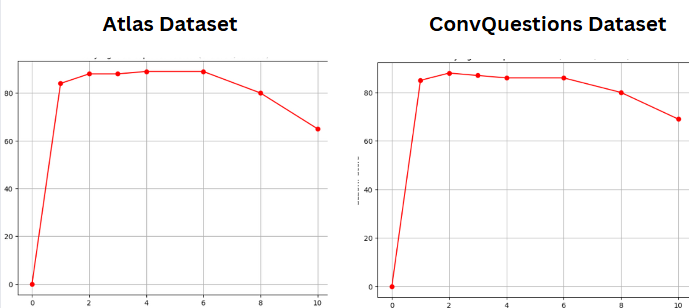
\includegraphics[width=1\linewidth]{figures/fusion.png}
    \caption{Comparison of BERTScore across different datasets with varying values of K for top K fusion.}
    \label{fig:fusion}
\end{figure}

The results revealed a unique trend in the \( K \)-vs-quality curve. Initially, as \( K \) increased, the quality of the answers improved. However, after reaching a certain threshold, further increases in \( K \) led to a sharp decline in quality. This trend was observed in both the ranked and random fusion strategies, although the ranked fusion consistently outperformed the random fusion at every \( K \).

\begin{itemize}
    \item \textbf{Quality}: For both strategies, the quality improved as \( K \) increased initially, but after a certain point, the quality degraded sharply with larger \( K \). This suggests that beyond a certain number of fused responses, adding more models leads to a dilution of quality, likely due to conflicting or less relevant model outputs.
    \item \textbf{Latency}: The latency increased linearly with \( K \), as more responses needed to be processed and fused.
\end{itemize}

\subsubsection{Observations}
The experiments highlighted the following insights:
\begin{itemize}
    \item Ranking is critical for optimizing the fusion process. Even though random fusion can provide some speedup, it leads to a noticeable drop in quality compared to ranked fusion.
    \item The quality improvement with increasing \( K \) follows a bell-shaped curve. While increasing \( K \) initially improves answer quality, fusing too many responses can degrade it.
    \item Ranking is a computationally expensive operation but is essential to maintain high-quality answers, particularly as \( K \) increases. This reinforces the importance of ranking in fusion strategies.
\end{itemize}



\section{Conclusion}
In this work, we explored the dynamic nature of large language model (LLM) performance across varying conversational contexts and proposed several strategies to optimize the ensembling of LLM responses. Our experiments demonstrated that no single LLM consistently outperforms others across different topics, highlighting the necessity of employing a diverse set of LLMs to ensure comprehensive coverage of various conversational themes. This finding underscores the importance of dynamic ensembling techniques, which allow us to adaptively select LLMs based on their contextual strengths.

We also investigated various strategies to avoid full ranking while balancing response quality and latency. Our findings revealed that while full ranking yields the highest quality of responses, it incurs substantial computational costs. In contrast, strategies such as Fixed-Interval Elimination provide significant speedup but at the cost of response quality. Dynamic Question-Specific Elimination emerged as a promising approach, maintaining a high-quality output while achieving substantial latency reductions.

Additionally, our examination of the impact of the parameter \( K \) on the fusion of responses from multiple LLMs indicated that an optimal number of models should be chosen for fusion to maximize response quality. While increasing \( K \) can enhance quality initially, our results suggest that beyond a certain threshold, the inclusion of additional LLM responses can lead to a degradation in quality.

Overall, this research contributes to the understanding of LLM behavior in conversation and highlights the importance of adaptable ensembling strategies. Future work may focus on refining these strategies further and exploring additional strategies that could enhance the overall performance of LLM ensembles in real-world applications.



\section{Acknowledgments}

Identification of funding sources and other support, and thanks to
individuals and groups that assisted in the research and the
preparation of the work should be included in an acknowledgment
section, which is placed just before the reference section in your
document.

This section has a special environment:
\begin{verbatim}
  \begin{acks}
  ...
  \end{acks}
\end{verbatim}
so that the information contained therein can be more easily collected
during the article metadata extraction phase, and to ensure
consistency in the spelling of the section heading.

Authors should not prepare this section as a numbered or unnumbered {\verb|\section|}; please use the ``{\verb|acks|}'' environment.

\section{Appendices}



\section{SIGCHI Extended Abstracts}

The ``\verb|sigchi-a|'' template style (available only in \LaTeX\ and
not in Word) produces a landscape-orientation formatted article, with
a wide left margin. Three environments are available for use with the
``\verb|sigchi-a|'' template style, and produce formatted output in
the margin:
\begin{description}
\item[\texttt{sidebar}:]  Place formatted text in the margin.
\item[\texttt{marginfigure}:] Place a figure in the margin.
\item[\texttt{margintable}:] Place a table in the margin.
\end{description}

%%
%% The acknowledgments section is defined using the "acks" environment
%% (and NOT an unnumbered section). This ensures the proper
%% identification of the section in the article metadata, and the
%% consistent spelling of the heading.
\begin{acks}
To Robert, for the bagels and explaining CMYK and color spaces.
\end{acks}

%%
%% The next two lines define the bibliography style to be used, and
%% the bibliography file.
\bibliographystyle{ACM-Reference-Format}
\bibliography{references}


%%
%% If your work has an appendix, this is the place to put it.
\appendix

\section{Research Methods}

\subsection{Part One}

Lorem ipsum dolor sit amet, consectetur adipiscing elit. Morbi
malesuada, quam in pulvinar varius, metus nunc fermentum urna, id
sollicitudin purus odio sit amet enim. Aliquam ullamcorper eu ipsum
vel mollis. Curabitur quis dictum nisl. Phasellus vel semper risus, et
lacinia dolor. Integer ultricies commodo sem nec semper.

\subsection{Part Two}

Etiam commodo feugiat nisl pulvinar pellentesque. Etiam auctor sodales
ligula, non varius nibh pulvinar semper. Suspendisse nec lectus non
ipsum convallis congue hendrerit vitae sapien. Donec at laoreet
eros. Vivamus non purus placerat, scelerisque diam eu, cursus
ante. Etiam aliquam tortor auctor efficitur mattis.

\section{Online Resources}

Nam id fermentum dui. Suspendisse sagittis tortor a nulla mollis, in
pulvinar ex pretium. Sed interdum orci quis metus euismod, et sagittis
enim maximus. Vestibulum gravida massa ut felis suscipit
congue. Quisque mattis elit a risus ultrices commodo venenatis eget
dui. Etiam sagittis eleifend elementum.

Nam interdum magna at lectus dignissim, ac dignissim lorem
rhoncus. Maecenas eu arcu ac neque placerat aliquam. Nunc pulvinar
massa et mattis lacinia.

\end{document}
\endinput
%%
%% End of file `sample-sigconf-authordraft.tex'.
